\documentclass{llncs}

\usepackage[english]{babel}
\usepackage[T1]{fontenc}  
\usepackage[utf8]{inputenc}
\usepackage[usenames,dvipsnames,table]{xcolor}
\bibliographystyle{splncs}
\usepackage{url}
%\usepackage[section]{placeins}

\usepackage{verbatim}
\usepackage{graphicx}
\usepackage{booktabs}
%\usepackage{chngpage}
\usepackage{fancyhdr}
%\usepackage{algorithm}
%\usepackage{algpseudocode}
%\usepackage{algorithmicx}
\setcounter{secnumdepth}{3}
\setcounter{tocdepth}{3}

\pagestyle{fancy}
\renewcommand{\headrulewidth}{0pt}

\lhead{\color{gray}\footnotesize ECAC- Error detection in transaction's data}
\rhead{\color{gray}\footnotesize José Pedro Marques, Tiago Pereira}
\lfoot{\color{gray}\footnotesize \rightmark}
\rfoot{\color{gray} \footnotesize Page. \thepage} 
\cfoot{}

\begin{document}

\title{SSIM TITLE}
\subtitle{Intelligent Systems, Interaction and Multimedia Seminar}
\author{José Pedro Marques, André Maia}
\institute{Faculdade de Engenharia da Universidade do Porto}
\date{November 11, 2012}
\maketitle


\begin{abstract}
Data Mining is a very broad area, with several algorithms applicable to the same problem. The purpose of this paper is to show a framework that given a specific problem as input, solves it using the best possible algorithm. To reach this goal, a distributed multi-agent system that tries to negotiate the best approach to each problem will be implemented, and this system will be tested with the data from the Portuguese Institute of Statistics, on an error detection problem.
\end{abstract}


\section{Introduction}

The purpose of this article is to present the framework that will be developed, as well as all the protocols that will be implemented. To best demonstrate the inner workings of the framework, a specific problem was chosen.

This article will include a description of the problem, the data available (Section 2.2) and it's difficulties (Section 2.3). This is followed by a description of the chosen algorithms (Section 2.4).

\section{The Problem}

\subsection{Description}

The information from each transaction a Portuguese company makes with an EU country reaches the Portuguese Institute of Statistics(INE) through the INTRASTAT form. In this form, the company provides information  about the transaction type (import/export), the item id, the weight of goods traded, the total cost, etc. Then this data is manually inserted into a database at INE. Figure 1 presents an excerpt of the data.

As in all manual processes, both the form filling and the insertion in the database are error prone, which could lead to incorrect/inconsistent data. For instance, an incorrectly introduced item id will associate a transaction with the wrong item. While some errors may be irrelevant to some statistics, some errors can influence them greatly.

Therefore, when all of the transactions relative to a month have been entered into the database, they are manually verified with the aim of detecting and correcting as many errors as possible. In this search, the experts try to detect unusual values in the values that describe the transactions.
Given that the number of transactions declared monthly is in the order of tens of thousands, this is a very costly process.

The idea then is to automatically select a subset of the transactions that includes almost all the errors that the experts would detect by looking at all the transactions.

\subsection{Data}

The data is organized in 2 files per month, one with the outgoing transactions and one with the incoming. Each line is a transaction, with 18 attributes, such as item id, price paid, weight, etc. The last attribute is a boolean attribute error, which indicates if that transaction contains (or not) an error.

\subsection{Difficulties}

One of the problems with the data is related to the attribute "weight", as it might contain null values when the weight of an item as less than a given threshold. But the biggest difficulty we will face is
the obviously unbalanced classes, as we expect only a few errors in the totality of the transactions. Therefore, the algorithms must be carefully chosen, having this problem in mind.

\subsection{Chosen Algorithms}

\subsubsection{Clustering for Outlier Detection}
This technique is not usually used for outlier detection, but it can be used for that task.
Every value assigned to a small cluster containing significantly fewer points than the others, is considered an outlier.

\subsubsection{Decision Trees for Outlier Detection}
Algorithms based on decision trees, learn from a set of pre-classified examples, and build a model of the regularities found used to classify new cases.
This kind of technique is better suited for the detection of outliers, where an isolated branch is classified has an outlier.
This is an algorithm that as the advantage that it doesn't require the need to define the number of clusters, and it is not scalable, this is, he's complexity over time is he's numbers of objects (O(n*n)). Although the interpretation of results can be subjective.

\subsubsection{Cell based outlier detection}
This algorithm can be described has a fast outlier detection algorithm for large datasets. This algorithm can avoid large computations on the majority part of dataset by filtering the initial dataset.
A large dataset is loaded into memory by blocks, and the data are placed into appropriate cells based on their values. Each cell holds a certain number of data, which represents the cell's density. Data located in high density cells who have no nearness relationship with local outlier factor calculation are filtered. And we record these cells density for the next block of data filled in. The final calculation will be done on those data in low density cells. This way, we can handle a large dataset which can't be loaded into memory all at once, improving the algorithm's efficiency by reducing many useless computations. The time complexity is O(N).


\section{The Framework}

\subsection{Architecture}

The Market will be implemented as a web-service, to facilitate the distribution of the whole process. Each agent then communicates with the Market as depicted in figure \ref{fig:marketArc}. 
\begin{figure}
\centering
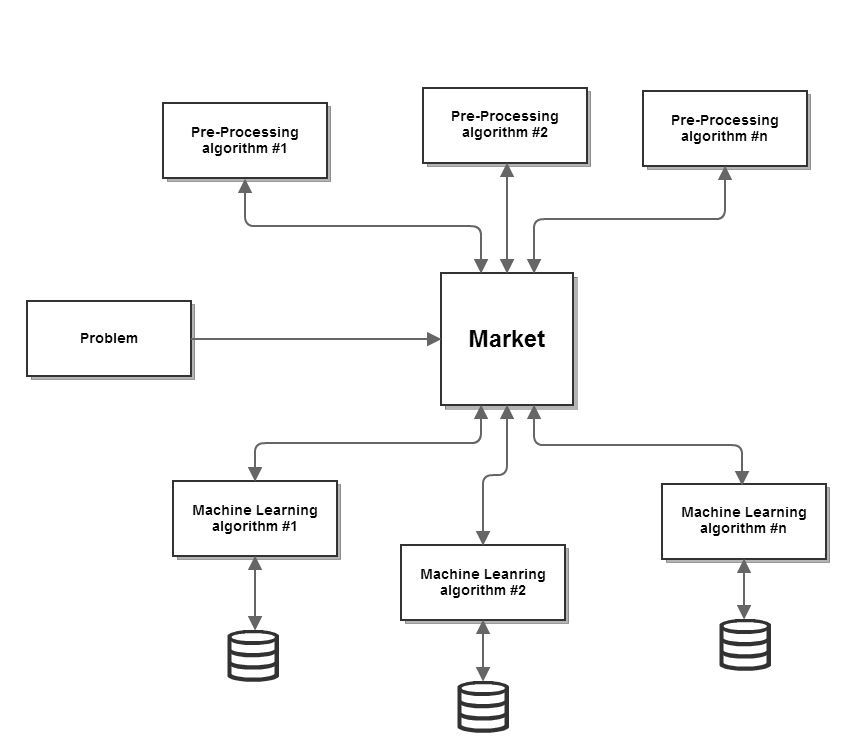
\includegraphics[width=\linewidth]{SSIM_architecture}
\caption{System Architecture}
\label{fig:marketArc}
\end{figure}


\subsection{Agents}

Each algorithm will be implemented as an independent agent, that communicates with the market. 

The pre-processing algorithms will receive the raw problem data as input and are responsible for cleaning the data (remove duplicates, remove nulls, date conversion, etc.), while each Machine Learning algorithm will receive the clean versions of the data and try to solve the problem. 





\subsection{Negotiation Process}




\section{Technology}

The Market will be implemented in Ruby on Rails \cite{tec:RoR} and each agent will be implemented in Java, with the help of JRI \cite{tec:JRI}, to make use of the already implemented algorithms in R \cite{tec:R}

The communication between the Market and each agent will follow the REST architecture \cite{tec:REST} through JSON \cite{tec:JSON} messages.

\begin{thebibliography}{9}
\bibitem{art:scc}
Soares, Costa, Cortez, Cavalho - Error Detection in Foreign Trade Data   using Statistical and Machine Learning Algorithms

\bibitem{tec:RoR}
Ruby on Rails:
\url{http://rubyonrails.org/}

\bibitem{tec:JRI}
JRI - Java/R Interface : 
\url{http://www.rforge.net/JRI/}

\bibitem{tec:R}
The R Project for Statistical Computing :
\url{http://www.r-project.org/}

\bibitem{tec:REST}
Representational State Transfer (REST) :
\url{http://www.ics.uci.edu/~fielding/pubs/dissertation/rest_arch_style.htm}

\bibitem{tec:JSON}
JSON :
\url{http://www.json.org/}



\end{thebibliography}

\end{document}
